

%%%%%%%%%%%%%%%%%%%%%%%%%%%%%%
% 	   美赛模板,正文部分		 
%          PAPER.tex         
%%%%%%%%%%%%%%%%%%%%%%%%%%%%%%

\documentclass[12pt]{article}

% 请在此填写控制号、题号和标题,年份不需要填(自动以当前电脑时间年份为准)
\usepackage[1902639]{easymcm}\problem{C}  
\usepackage{cite} 
\usepackage{url}
\usepackage{subfigure}
\usepackage{palatino} % 这个是COMAP官方杂志采用的字体,如不需要可注释掉,以使用默认字体
\title{Analysis and Strategies to the Opioids Crisis }  % 标题

% 如您参加的是ICM(即选择了D/E/F题),请使用以下的命令修改Summary Sheet题头
% \renewcommand{\contest}{Interdisciplinary Contest in Modeling (ICM) Summary Sheet}

% 正文开始
\begin{document}
%%%%%%%%%%%%%%%%%%%%%%%%%%%%%%%%%%%%%%%%%
%%            请在此填写摘要            %%
%% 请勿编译/排版此文件,请编译PAPER.tex!  %%
%%%%%%%%%%%%%%%%%%%%%%%%%%%%%%%%%%%%%%%%%
\begin{abstract}\small
    Here is the abstract of your paper.

    Firstly, that is ...

    Secondly, that is ...
We analyze the correlation between drug identification counts socio-economic factors by Apriori, which is an algorithm for frequent item set mining and association rule learning over transactional databases. From the result, we draw a conclusion that adults with some college education and with no education beyond high school who don't get married, men with no wife present and women with no husband and own children present are likely to use/abuse opioids, and the growth of its percentage contributes to the growth of the percentage of opioid use and addiction. 
    Finally, that is ...

    % 美赛论文中无需注明关键字。若您一定要使用,
    % 请将以下两行的注释号'%'去除,以使其生效;
    % 若您不使用,可直接将这段注释删除
    \vspace{5pt}
    \textbf{Keywords}: MATLAB, mathematics, LaTeX.

Governor Jay Inslee 

Office of the Governor 

PO Box 40002

Olympia, WA 98504-0002 

Dear Governor Inslee:

I write to you on behalf of the MCM team 1902639. We are extremely concerned about the opioid crisis in the United States. Investigation shows that opioid use and addiction have spread among a large number of states and counties. We hope to help you improve the traffic conditions.

Opioid use and addiction could bring about health and major economy problems. Firstly, opioids lead to a large number of negative health, such as opioid use disorder, hepatitis, and HIV infections, and neonatal abstinence syndrome. Secondly, opioids overdoes can lead to death. Thirdly, it will be difficult to fill positions of high-tech and reliable workers if the crisis spreads to special population such as the high-educated. Lastly, if the percentage of people with opioid addiction increases within the elderly, it will affect the health care costs and assisted living facility staffing.

After an in-depth study of the drug conditions in 5 states (Ohio, Pennsylvania, Virginia, West Virginia and Kentucky), we have come up with some ideas that can help address this issue.

Sincerely yours

MCM 2019 Team 1902639
\end{abstract}



%%%%%%%%%%%%%%%%%%%%%%%%%%%%%%%%%%%%%%%%%%
% 如不理解以下部分中各命令的含义,请勿修改! %
%%%%%%%%%%%%%%%%%%%%%%%%%%%%%%%%%%%%%%%%%%

%---------以下生成sheet页----------
% 下面的语句可调整全文行距为标准值的0.6倍,请自行使用
% \renewcommand{\baselinestretch}{0.6}\normalsize
\maketitle  			% 生成sheet页
\thispagestyle{empty}   % 不要页眉页脚和页码
\setcounter{page}{-100} % 此命令仅是为了避免页码重复报错,不要在意

%---------以下生成目录----------
\newpage
\tableofcontents
\thispagestyle{empty}   % 不要页眉页脚和页码
\newpage

%---------以下生成正文----------
\setlength\parskip{0.8\baselineskip}  % 调整段间距
\setcounter{page}{1}    % 从正文开始计页码
\pagestyle{fancy}		% 摘要请到ABSTRACT.tex中填写


\section{Restatement of the Problem}
\subsection{Background}
\subsubsection{An Overview of the Problem}
In recent years, as the crisis regarding the use of synthetic and non-synthetic opioids is upgrading, American governments has attached great significance to the cure for addiction and the prevention of opioids. A meaningful part of the opioid control is to analyze drug identification counts itself and its correlation with socio-economic factors. By this way, we can throw out reasonable strategies to help counter the crisis. Data for counties of 5 states (Ohio, Pennsylvania, Virginia, West Virginia and Kentucky) in years 2010-2016/2017 is provided by DEA/NFLIS and USCB.

There are several health and major economy problems in the opioids crisis. Firstly, opioids lead to a large number of negative health, such as opioid use disorder, hepatitis, and HIV infections, and neonatal abstinence syndrome. Secondly, opioids overdoes can lead to death. Thirdly, it will be difficult to fill positions of high-tech and reliable workers if the crisis spreads to special population such as the high-educated. Lastly, if the percentage of people with opioid addiction increases within the elderly, it will affect the health care costs and assisted living facility staffing. Therefore it makes great sense to handle the opioid crisis.

\subsubsection{Literature Review}
Opioids are a class of drugs used to reduce pain, including approximately 3 groups\cite{CDC}. The first group is prescription opioids, whose common types are oxycodone, hydrocodone, morphine, and methadone. The second group is a synthetic opioid pain reliever called fentanyl, which is many times more powerful than other opioids but is approved for treating. As a result, illegally made and distributed fentanyl is an acute problem which is hard to manage by the government\cite{fentanyl}. The third group is heroin, which is illegal but, in fact, never disappear around the country\cite{heroin}.

Drugs including opioids have been a major problem plaguing the American Society for a long time, and it tends to become much more acute in recent years. The number of drug overdose deaths has never been higher, and the majority among these deaths, 68 \% in 2017, involved opioids \cite{overdose}. 



\subsection{Our work}
Our tasks at hand are listed as follows:
\begin{itemize}
    \item Construct a mathematical model to simulate the spread of the synthetic opioid and heroin cases in and between the five states and their counties over time, describe the characteristics, and identify some possible locations where specific opioid use might have started in each of the five states. 
    \item On the basis of the patterns and characteristics we identified, give some policy suggestions to improve the situation. Predict the drug identification threshold levels and the place and date it will occur.
    \item Propose some modifications from socio-economic data to include some important factors which can explain how opioid use got to its current level, who is using/abusing it, what contributes to the growth in opioid use and addiction, why opioid use persists despite its known dangers, whether use or trends-in-use is associated, and so on. 
    \item On the basis of the modified model, identify a possible strategy for countering the opioid crisis. Test the effectiveness of this strategy and identify some significant parameter bounds.
\end{itemize}


\section{Preparation of the Models}
\subsection{Assumptions and Justifications}
In order to simplify the course of modeling and draw some reasonable conclusions from our model, we make assumptions as follows:
\begin{itemize}
	\item The dataset offered is accurate and 
	\item 
	\item 
\end{itemize}

\subsection{Notations}
The primary notations and symbols used in this paper are listed in \textbf{Table \ref{tb:notation}}. Some of them will be defined later in the following sections.
\begin{table}[!htbp]
\begin{center}
\caption{Notations}
\begin{tabular}{cl}
	\toprule
	\multicolumn{1}{m{3cm}}{\centering Symbol}
	&\multicolumn{1}{m{8cm}}{\centering Definition}\\
	\midrule
	$A$&the first one\\
	$b$&the second one\\
	$\alpha$ &the last one\\
	\bottomrule
\end{tabular}\label{tb:notation}
\end{center}
\end{table}


\section{Design of the Models}
\subsection{Spread Model}
In order to demonstrate our spread model clearly, we divide it into the following three sub models:
\begin{itemize}
	\item Self-spread model (SSD, Self Spread Death model): This model is designed to simulate the spread within each county. Cause the spread mechanism within a restricted place ( here we consider every single county to be a point) is quite similar to that of infectious diseases, we develop our self-spread model based on SIR epidemic models. Specially, we suppose self-spread and death caused by opioid overdose in this model, so we also call it 'SSD' model.
	\item Inter-spread model (QGS, Quasi Gradient-based Spread model): This model is designed to simulate the spread between counties. Enlightened by concentration gradient, we introduce the quasi gradient to quantify the population mobility. In the following writing, we also call this quasi gradient-based spread model as the 'QGS' model for convenience.
	\item Memory model: This model is introduced to reflect the inertia of the quantity change and reduce the influence of random noise and invalid data. We realize the memory ability by using a weighted combination of data from previous several years as our input.
\end{itemize}
\subsection{Correlation Analysis}
To find out the most influential factors to the opioid crisis among socio-economic data provided, we use the correlation analysis method to mine the data. Specifically, our mining algorithm is based on the Apriori algorithm. 

\section{The Basic Model}
Based on the given data, we found that the spread of drug identifications can be divided into two variations. On the one hand, the data changes at each certain location. On the other hand, it gradually spread to nearby areas. So we build these models to simulate the spread of opioids cases in the given five states. The self-spread model(SSD) simulates the changes of the opioids cases in a certain location and the inter-spread model simulate the geographical spread of the opioids cases. We also build a memory model to take the weight of time into consideration, which shows a better result.Using the models combined by the three sub models, we estimate the location where the opioids cases initially occur by backward-tracking and make a prediction on where it will happen in the future.
\subsection{Sub Models}
\subsubsection{Self-spread Model (SSD)}
Suppose the population $N$ doesn't change at each certain year, we can divide people into "opioids infectors” and “opioids susceptibles”. Given time t, the infection rate (the proportion of the infectors among the population) and the susceptible rate (susceptibles among the population) can be expressed as i(t),s(t). Each year there will be $\lambda N s$ people become infectors due to the influence of the existing infectors. Considering of the death rate of the infectors, there will be $\alpha N i$ infectors die of drugs. So we have:
\begin{equation}
\frac{\mathrm{d} i}{\mathrm{d} t} = \lambda si(1-\alpha)- \alpha i \text{,}\\ 
\end{equation}
\begin{equation}
\frac{\mathrm{d} s}{\mathrm{d} t}= - \lambda si(1-\alpha) \text{.}\\ 
\end{equation}
Solve the equation, we get the function curve of $i(t)$ and $s(t)$,which roughly show how i and s change over time(\textbf{Figure \ref{ist}}).

\begin{figure}[h]
\centering
\subfigure[{$i(t)$ and $s(t)$}]{
  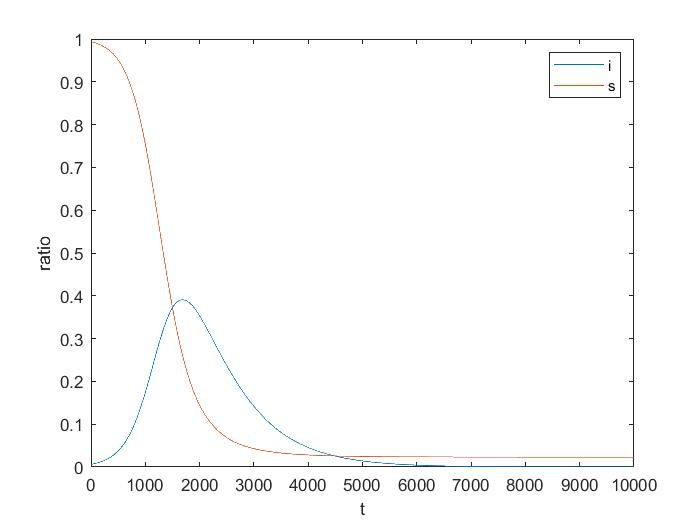
\includegraphics[scale=0.3]{plots/is-t.png}
}
\subfigure[{$i(t)$}]{
  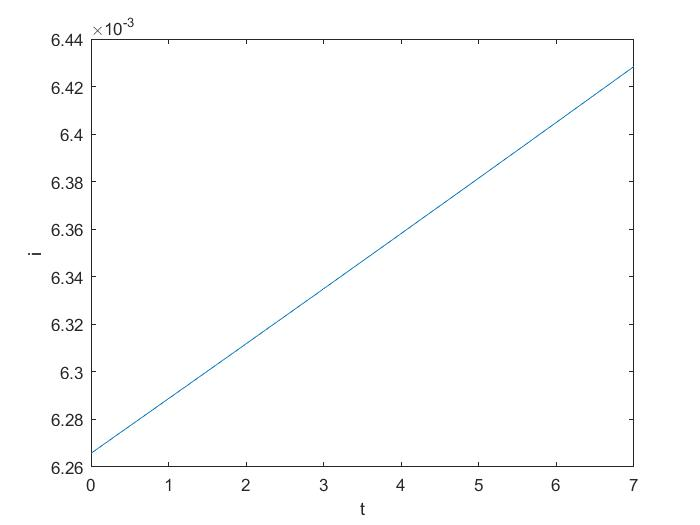
\includegraphics[scale=0.3]{plots/i-t,0-7.png}
}
\caption{$i(t)$ and $s(t)$}
\label{ist}
\end{figure}

We intercept the values when ranging from 1 to 7 and the curve indicates I have a very good linear correlation with t. Reasonably, we assume i have a linear correlation with t.So the $\lambda$ can be estimated at the point t=0, which indicate that
\begin{equation}
\end{equation}

Then we make a linear regression with the average infection rate during 2010-2016(we remain the data of 2017 to test the accuracy of our model. We use the slope of the curve as $\frac{\mathrm{d} i}{\mathrm{d} t}$, plug in equation(X) and we get the average $\lambda$ in each states (\textbf{Figure \ref{MFigure1} and Table \ref{lambda}}).

\begin{figure}[h]
\centering
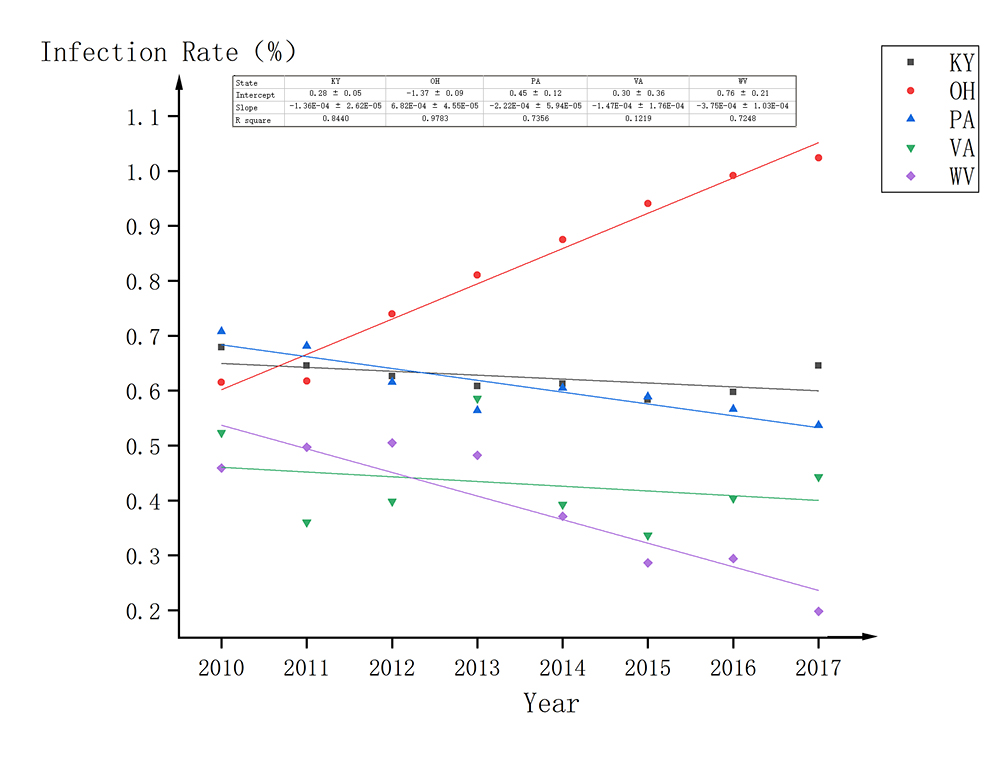
\includegraphics[width=10cm]{plots/MFigure1.png}
\caption{Infection Rate}
\label{MFigure1}
\end{figure}

\begin{table}[h]
\centering
\begin{tabular}{cccccc}
  \toprule
   & \multicolumn{5}{c}{State} \\
  \cmidrule{2-6}
& KY & OH & PA & VA & WV  \\
  \midrule
  $\lambda$ & -1.90 & 11.3 & -3.03 & -2.70 & -8.09  \\
  \bottomrule
\end{tabular}
\caption{$\lambda$ value ($*10^{-2}$)}
\label{lambda}
\end{table}

\subsubsection{Inter-spread Model}
The infectors can move to other locations leading to the increase of the infection rate in other locations. In this will be more likely to choose a closer location as their their targets. So we assume the geographical spread of drug cases satisfies the gradient diffusion procedure.

where $\gamma$ is the diffusion coefficient.

\subsubsection{Memory Model}
Opioids cases spread over time, and we find that the distribution of the opioids cases in a certain year will have some similarity with that in the recent years. To reflect the inertia of the quantity change and reduce the influence of random noise and invalid data, we change the input form to realize the ability of 'memory'. More detailed, we realize the memory ability by using a weighted combination of data from previous several years as our input. The degree of similarity should be higher as the the time interval is shorter. We take the data from recent three years into our model and give them different weights. According to our tests, we choose 0.6, 0.3, 0.1 corresponding to the recent 1-3 years' data.

\subsection{Optimization}
\subsubsection{The optimization of $\gamma$}
Based on the three sub models, we set our precision as $10^-5$ to find the value of $\gamma$ and calculate the variance of the count of opioids cases in each state. Then we get the coefficient $\gamma$ corresponding to the minimal of the deviation(\textbf{Table \ref{gamma}}).

\begin{table}[h]
\centering
\begin{tabular}{cccccc}
  \toprule
   & \multicolumn{5}{c}{State} \\
  \cmidrule{2-6}
& KY & OH & PA & VA & WV  \\
  \midrule
  $\gamma$ & 11 & 0.3 & 7 & 4& 19  \\
  \bottomrule
\end{tabular}
\caption{$\gamma$ value ($*10^{-5}$)}
\label{gamma}
\end{table}

Using the $\lambda$ from SSD and $\gamma$ we have optimized, we set the number of opioids cases in 2010 as the initial value. The deviation of this model is as followed(\textbf{Table \ref{dev}}). 

\begin{table}[h]
\centering
\begin{tabular}{cccccccc}
  \toprule
   & \multicolumn{7}{c}{Year} \\
  \cmidrule{2-8}
& 2011 & 2012 & 2013 & 2014 & 2015 & 2016 & 2017  \\
  \midrule
KY & 0.0133 & 0.0096 & 0.0127 & 0.0120 & 0.0162 & 0.0168 & 0.0303 \\
OH & 0.1660 & 2.3111 & 2.2197 & 2.1813 & 1.6908 & 2.1505 & 3.3414 \\
PA & 0.3912 & 0.5782 & 1.3402 & 1.8634  & 0.9489 &  0.8898 & 0.8993 \\
VA & 0.1806 & 0.1880 & 0.0438 & 0.1489 & 0.1673 & 0.1539 & 0.1687 \\
WV & 0.0050 & 0.0059 & 0.0076 & 0.0054 & 0.0060 & 0.0054 & 0.0047 \\
  \bottomrule
\end{tabular}
\caption{Deviation of Results without Weight ($*10^{7}$)}
\label{dev}
\end{table}

\subsubsection{Apply the Memory Model}
Based on the optimized $gamma$ in 4.2.1, we apply the memory model(described in 4.1.3) to the current model. We regard the weighted count of opioids cases as the count of opioids cases the year before(e.g. use the weighted count of drug cases in 2012-2014 as the count of that in 2014 and get the result in 2015)(\textbf{Table \ref{dev2}}).

\begin{table}[h]
\centering
\begin{tabular}{cccccc}
  \toprule
   & \multicolumn{5}{c}{Year} \\
  \cmidrule{2-6}
& 2013 & 2014 & 2015 & 2016 & 2017  \\
  \midrule
  KY & 0.0751 & 0.1049 & 0.1193 & 0.0593 & 0.2373 \\
  OH & 3.1506 & 1.6764 & 1.8122 & 1.1424 & 3.1777 \\
  PA & 4.3250 & 4.1148 & 1.2450 & 1.1012 & 0.3884 \\
  VA & 1.8040 & 0.5481 & 0.3014 & 0.2166 & 0.1928 \\
  WV & 0.0554 & 0.0400 & 0.0342 & 0.0131 & 0.0399 \\
  \bottomrule
\end{tabular}
\caption{Deviations in Weighted Model ($*10^{7}$)}
\label{dev2}
\end{table}

As is shown in \textbf{Figure \ref{weigh}}, all the the deviations decrease compared to the former model (\textbf{Figure \ref{noweigh}}).The heat map of the value in 2013 and 2015 are shown in Figure,

\begin{figure}[h]
\centering
\subfigure[{Unweighted 2013}]{
  \label{no13}
  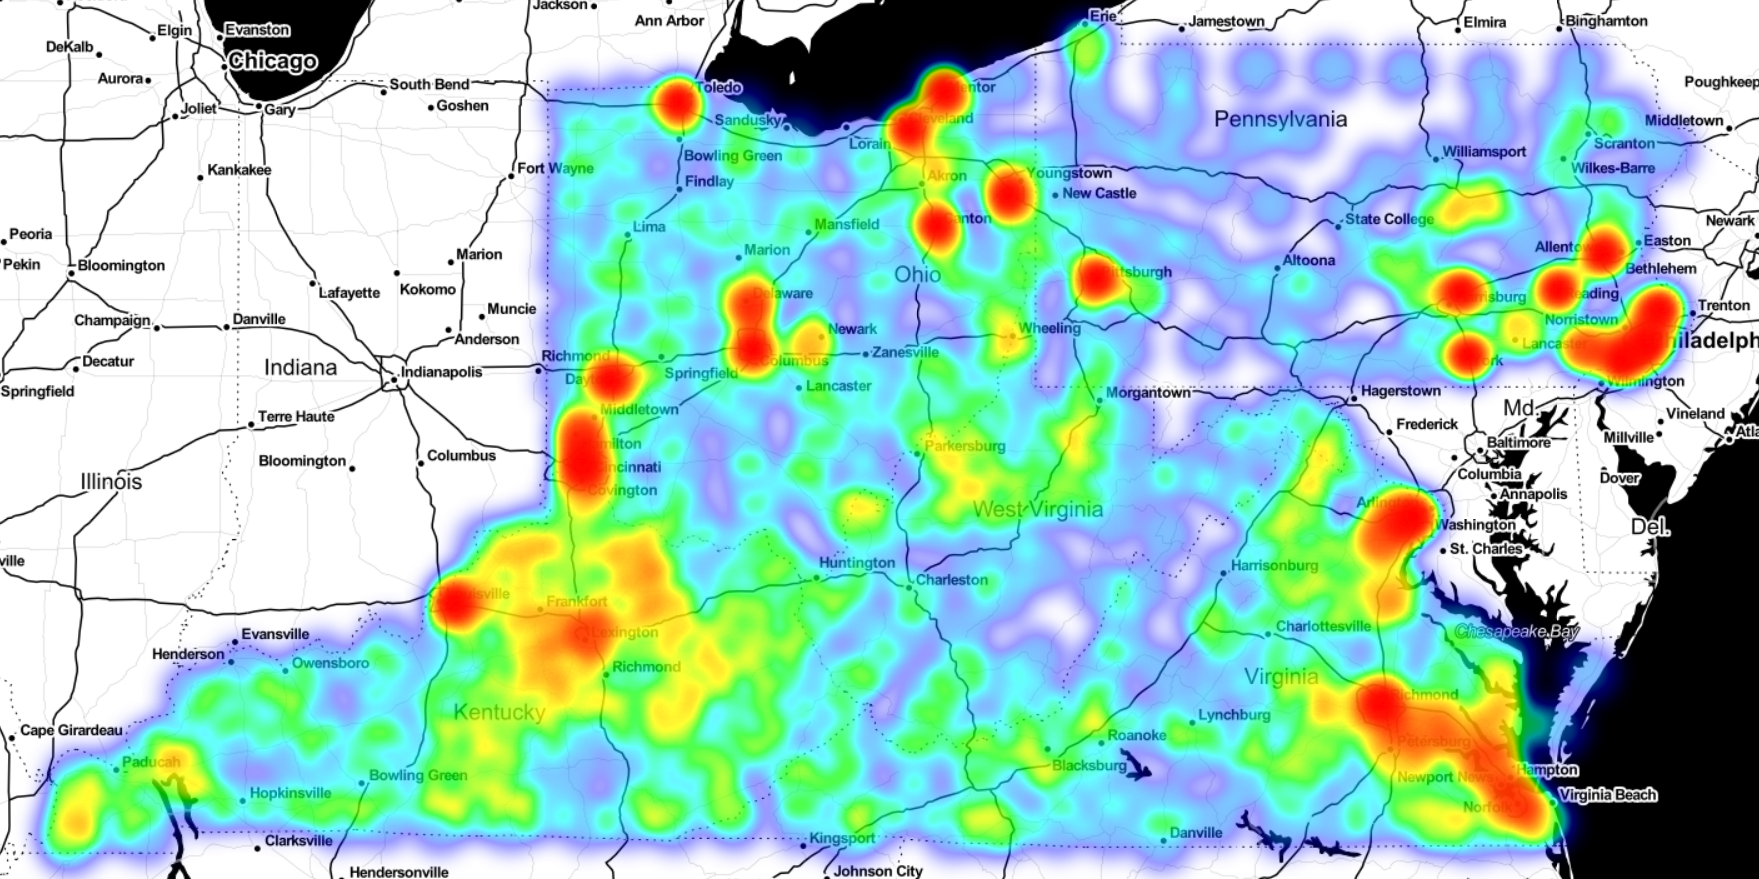
\includegraphics[scale=0.2]{plots/noweigh2013.png}
}
\subfigure[{Unweighted 2015}]{
  \label{no15}
  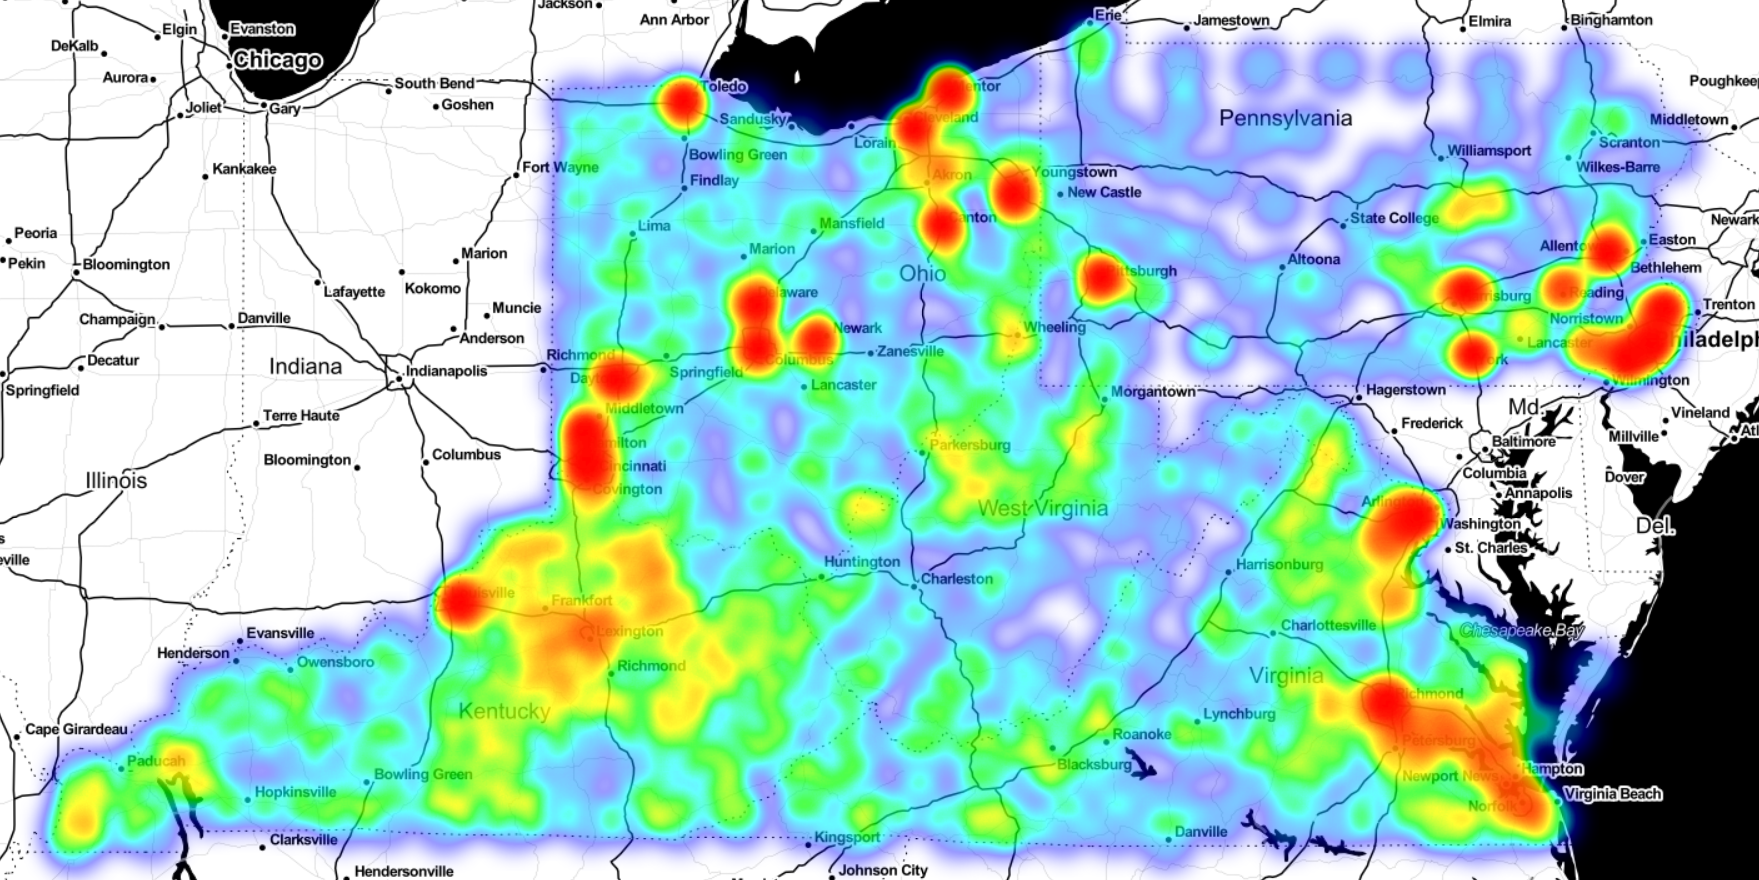
\includegraphics[scale=0.2]{plots/noweigh2015.png}
}
\caption{no weight}
\label{noweigh}
\end{figure}

\begin{figure}[h]
\centering
\subfigure[{Weighted 2013}]{
  \label{weigh13}
  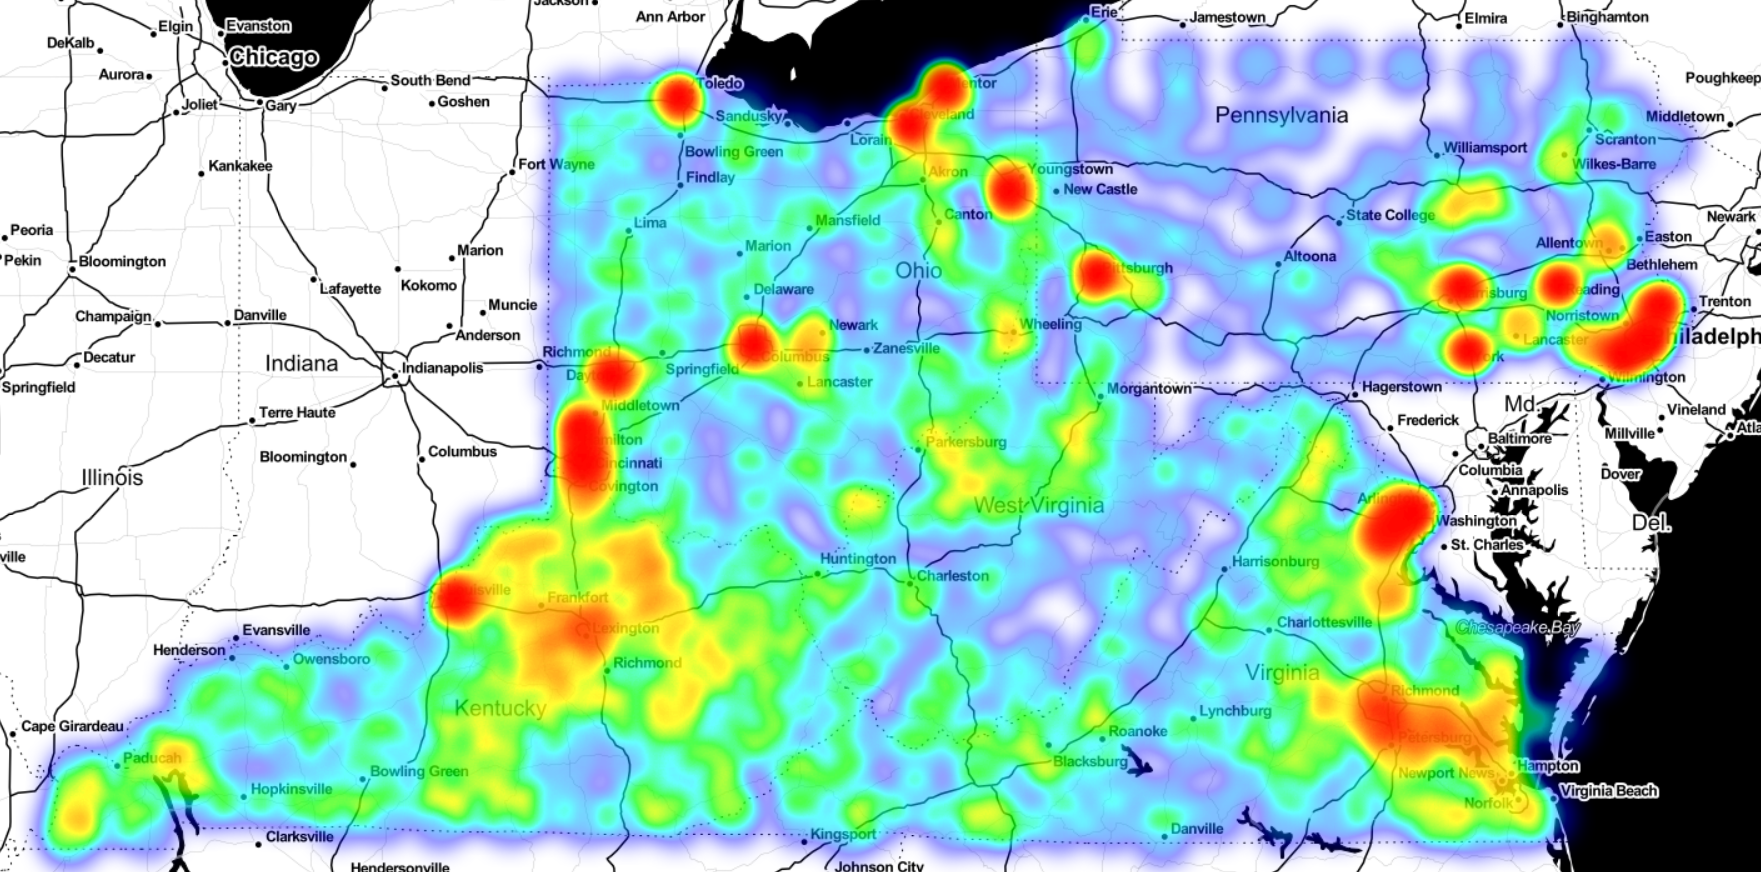
\includegraphics[scale=0.2]{plots/weigh2013.png}
}
\subfigure[{Weighted 2015}]{
  \label{weigh15}
  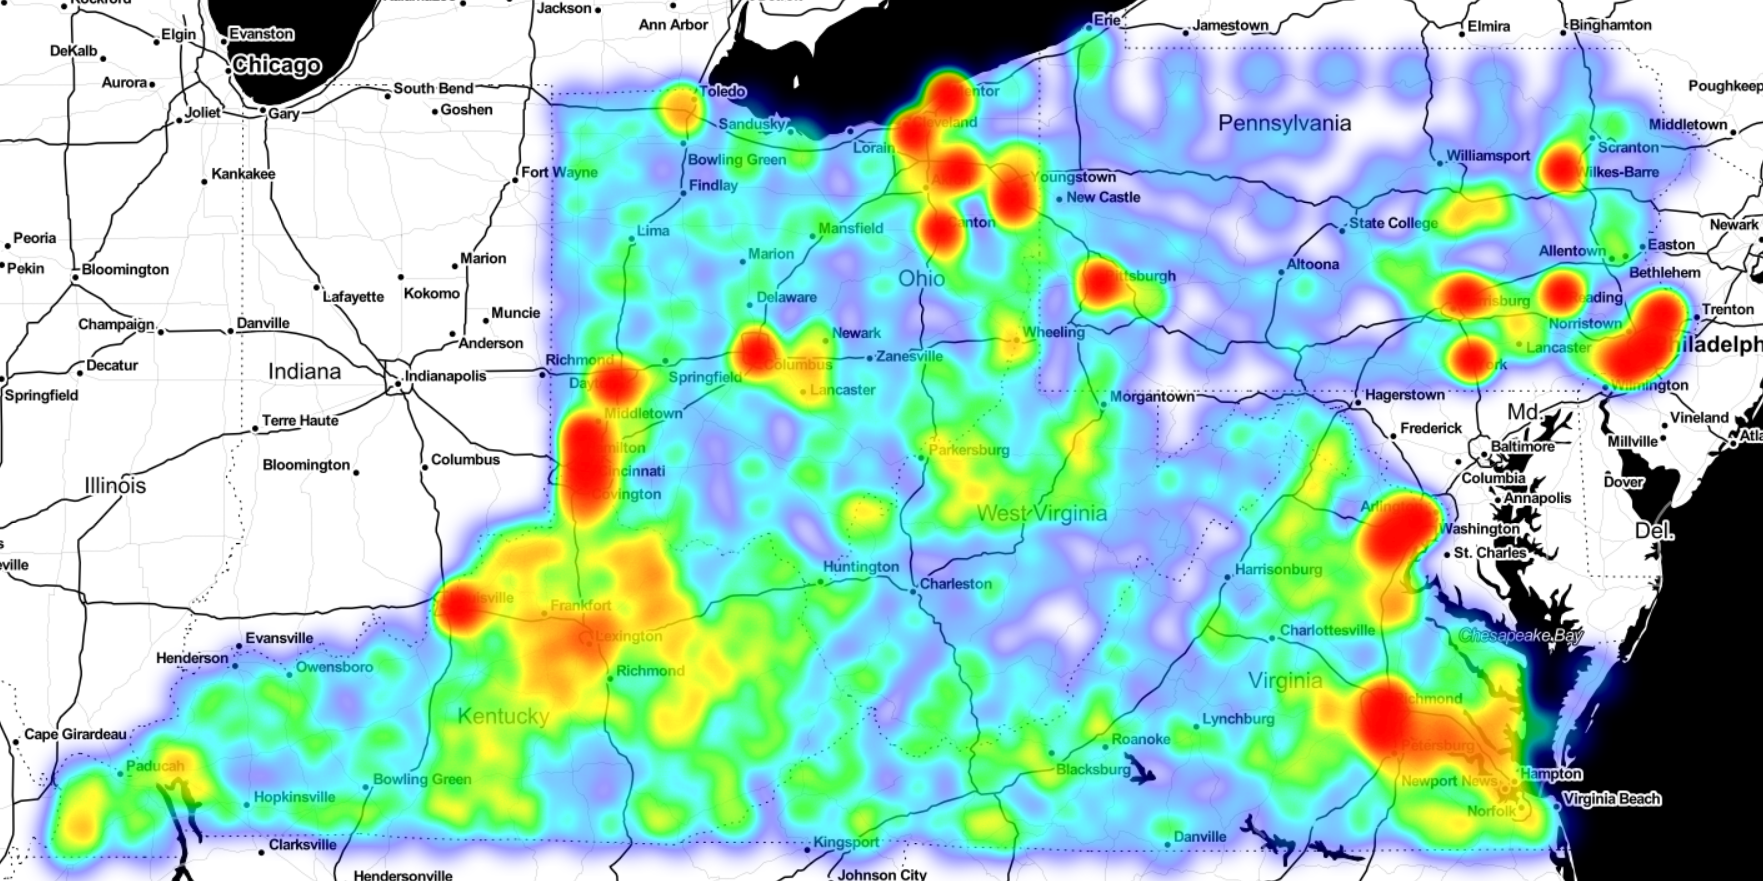
\includegraphics[scale=0.2]{plots/weigh2015.png}
}
\caption{Weighted}
\label{weigh}
\end{figure}

\subsection{Inferences Based on the Model}

\subsubsection{The Source of Opioids Cases}
In order to predict the source of opioids cases, we have to replace the coefficient $\gamma$ with some negative value, which indicates the locations of opioids cases will converge to several certain places. We choose the count of opioids cases in the year 2010,2011,2012(with weight 0.6, 0.3, 0.1) as the initial backtracking value and then regard the inferred count of opioid cases we get from following calculation as true value.

Noticing that the convergence speed is very slow if we simply replace $\gamma$ with $-\gamma$, we multiply $\gamma$ by -5000 and then we get a desirable result (\textbf{Figure \ref{iter} and Table \ref{infec}}).

\begin{figure}[h]
\centering
\subfigure[{iter15}]{
  \label{iter15}
  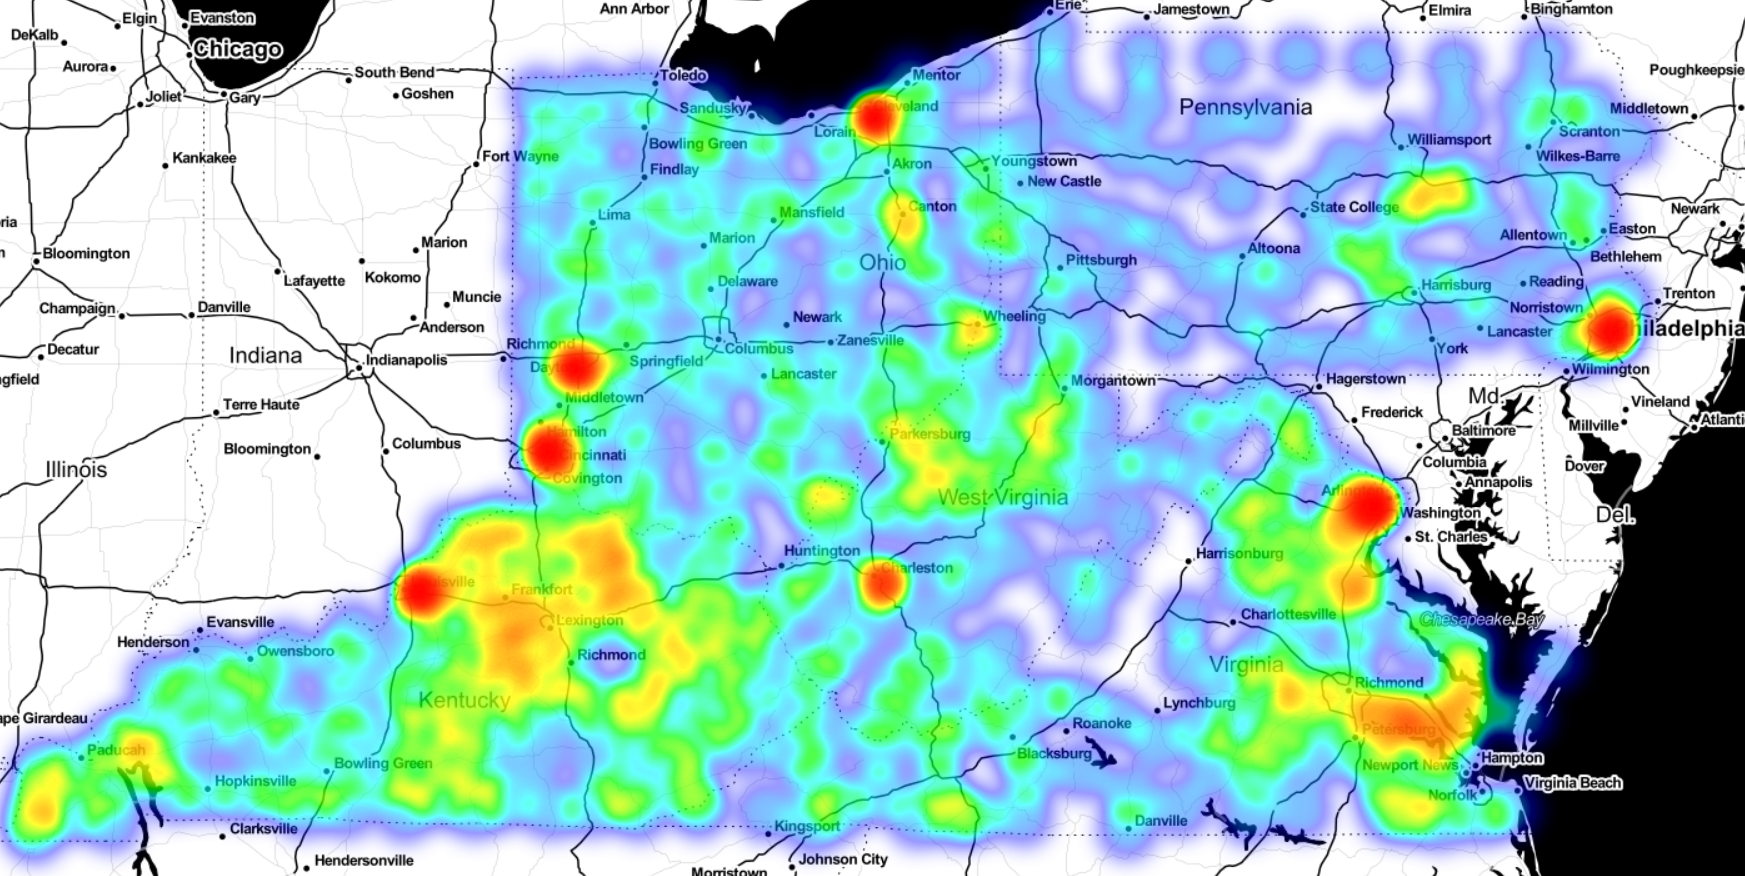
\includegraphics[scale=0.2]{plots/iteration15.png}
}
\subfigure[{iter30}]{
  \label{iter30}
  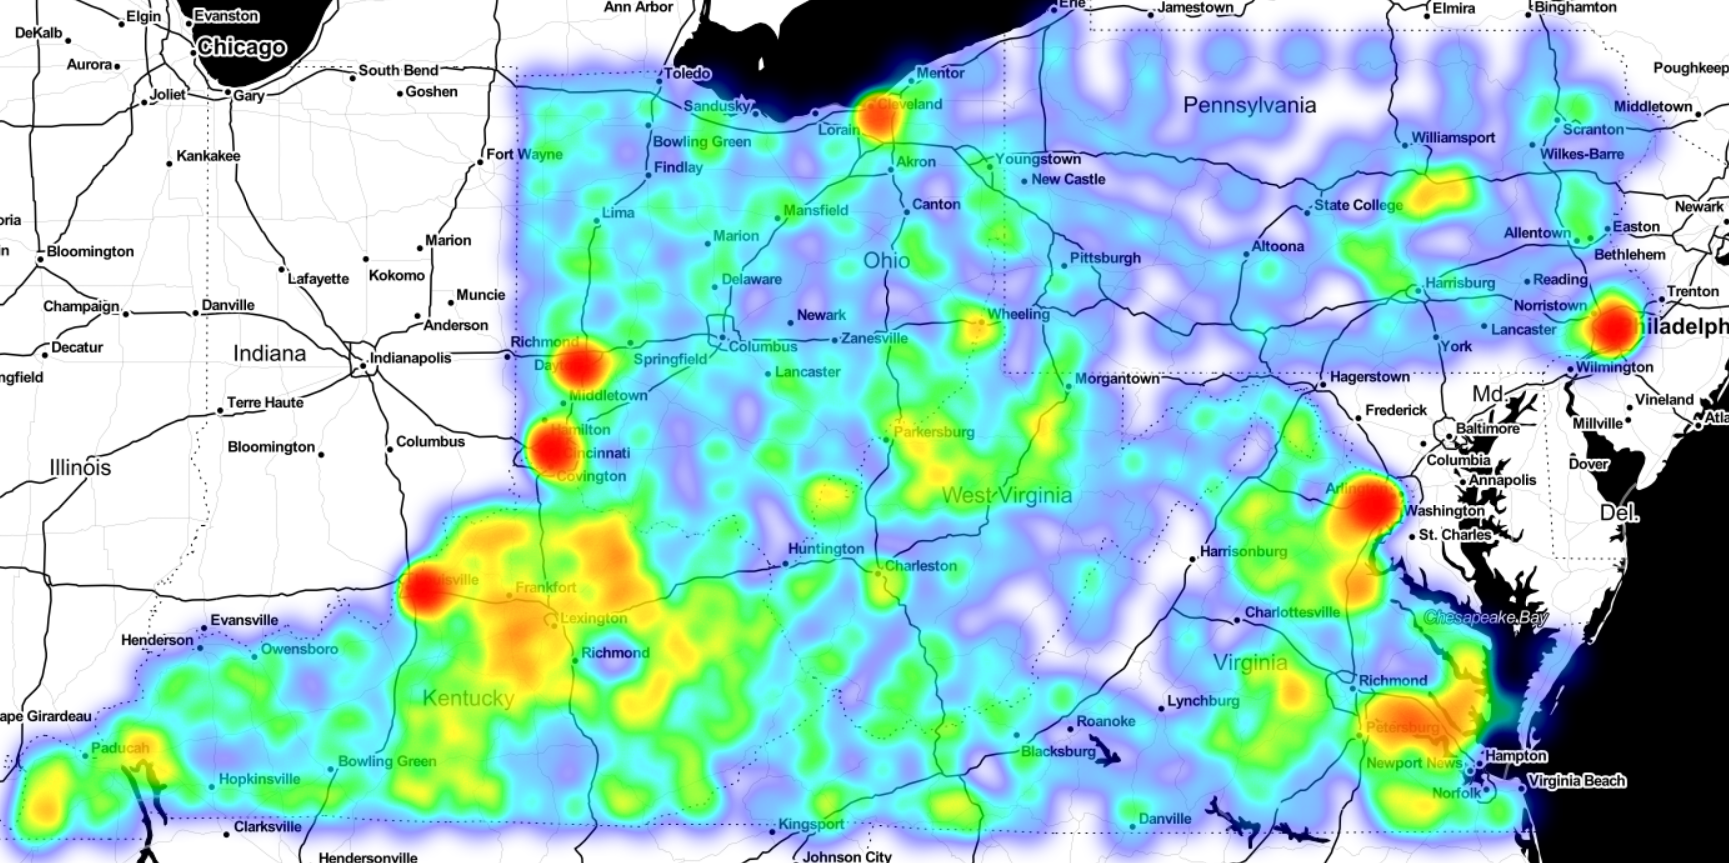
\includegraphics[scale=0.2]{plots/iteration30.png}
}
\caption{iter}
\label{iter}
\end{figure}

\begin{table}[h]
\centering
\begin{tabular}{cccccc}
  \toprule
State & County & Latitude & Longitude & Count &Iterations  \\
  \midrule
  KY &Jefferson &38.25 & -85.62&  5097.02 &>30 \\
KY &Fayette &38.03 & -84.44  &0 &11 \\
KY &Kenton &39.01  &-84.53 & 0 &5 \\
OH &Hamilton &39.20 & -84.51&  12380.12& >30 \\
OH &Montgomery &39.77  &-84.26& 9470.03& >30 \\
OH &Cuyahoga &41.44 & -81.62  &1946.39 &>30 \\
PA &Philadelphia &40.01 & -75.13  &28372.65& >30 \\
PA &Allegheny &40.46  &-79.98  &0 &15 \\
PA &Bucks &40.24 & -75.04 & 0 &7 \\
VA &Fairfax& 38.84 & -77.23  &2985.49& >30 \\
VA &Richmond &37.53 & -77.48 & 0 &24 \\
VA &Prince William& 38.70 & -77.43 & 0& 6 \\
VA &Chesterfield& 37.40 & -77.52  &0 &6 \\
WV &Kanawha &38.30 & -81.55 & 1572.98& >30 \\
WV &Berkeley &39.47 & -78.01&  0 &9 \\
WV &Mercer &37.37 & -81.16&  0 &6 \\
\bottomrule
\end{tabular}
\caption{Infection source analysis}
\label{infec}
\end{table}

\subsubsection{The Prediction}
In this case, we choose the latest count of opioids cases (from year 2016, 2015, 2014 with corresponding weight 0.6,0.3,0.1) as our initial value and $\lambda,\gamma$ in \textbf{Table \ref{lambda} and \ref{gamma}}. We use our spread model, and regard the inferred result as the true value(the same as we did in 4.3.1).

\begin{figure}[h]
\centering
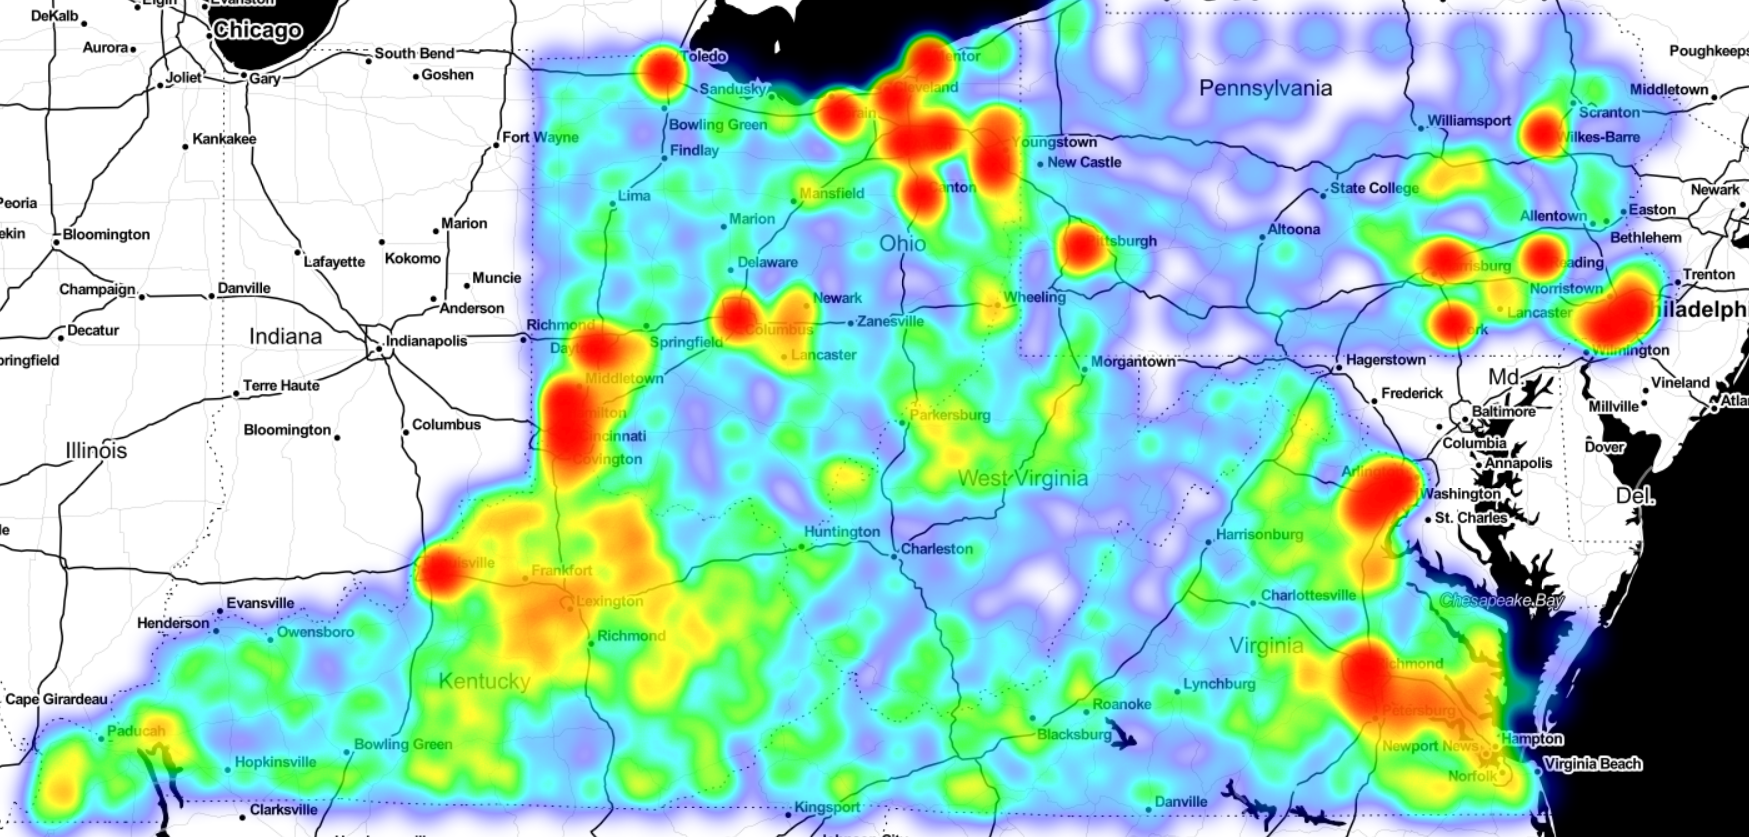
\includegraphics[width=10cm]{plots/prediction2017.png}
\caption{Prediction 2017}
\label{pre17}
\end{figure}

During this process we get the prediction of the count of opioids cases in 2017(\textbf{Figure \ref{pre17}}).We calculate its deviation from the true value (\textbf{Table \ref{dev2}}) and find advisable result.The results presented in heat map also shows the predicted distribution of opioids cases have a good similarity with the true distribution.
We continue our calculation process and get the predicted value in the next few years, the distribution of the predicted opioid cases are shown in the heatmap(\textbf{Figure \ref{pre}}).

\begin{figure}[h]
\centering
\subfigure[{Prediction 2020}]{
  \label{m-state}
  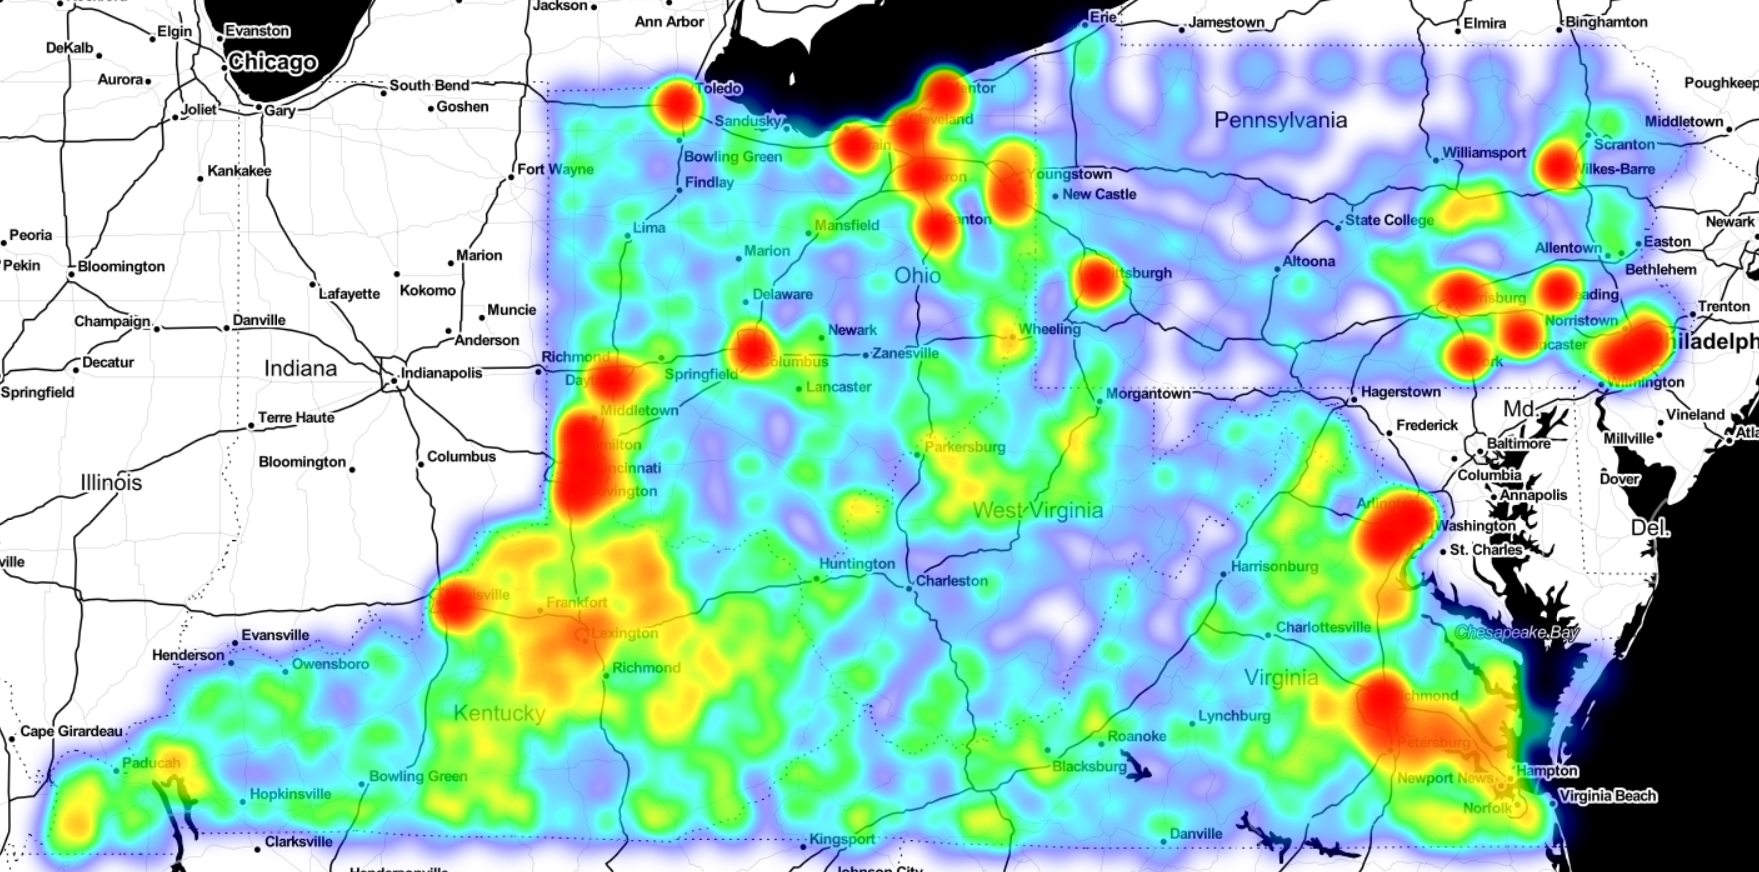
\includegraphics[scale=0.13]{plots/prediction2020.png}
}
\subfigure[{Prediction 2025}]{
  \label{mb-state}
  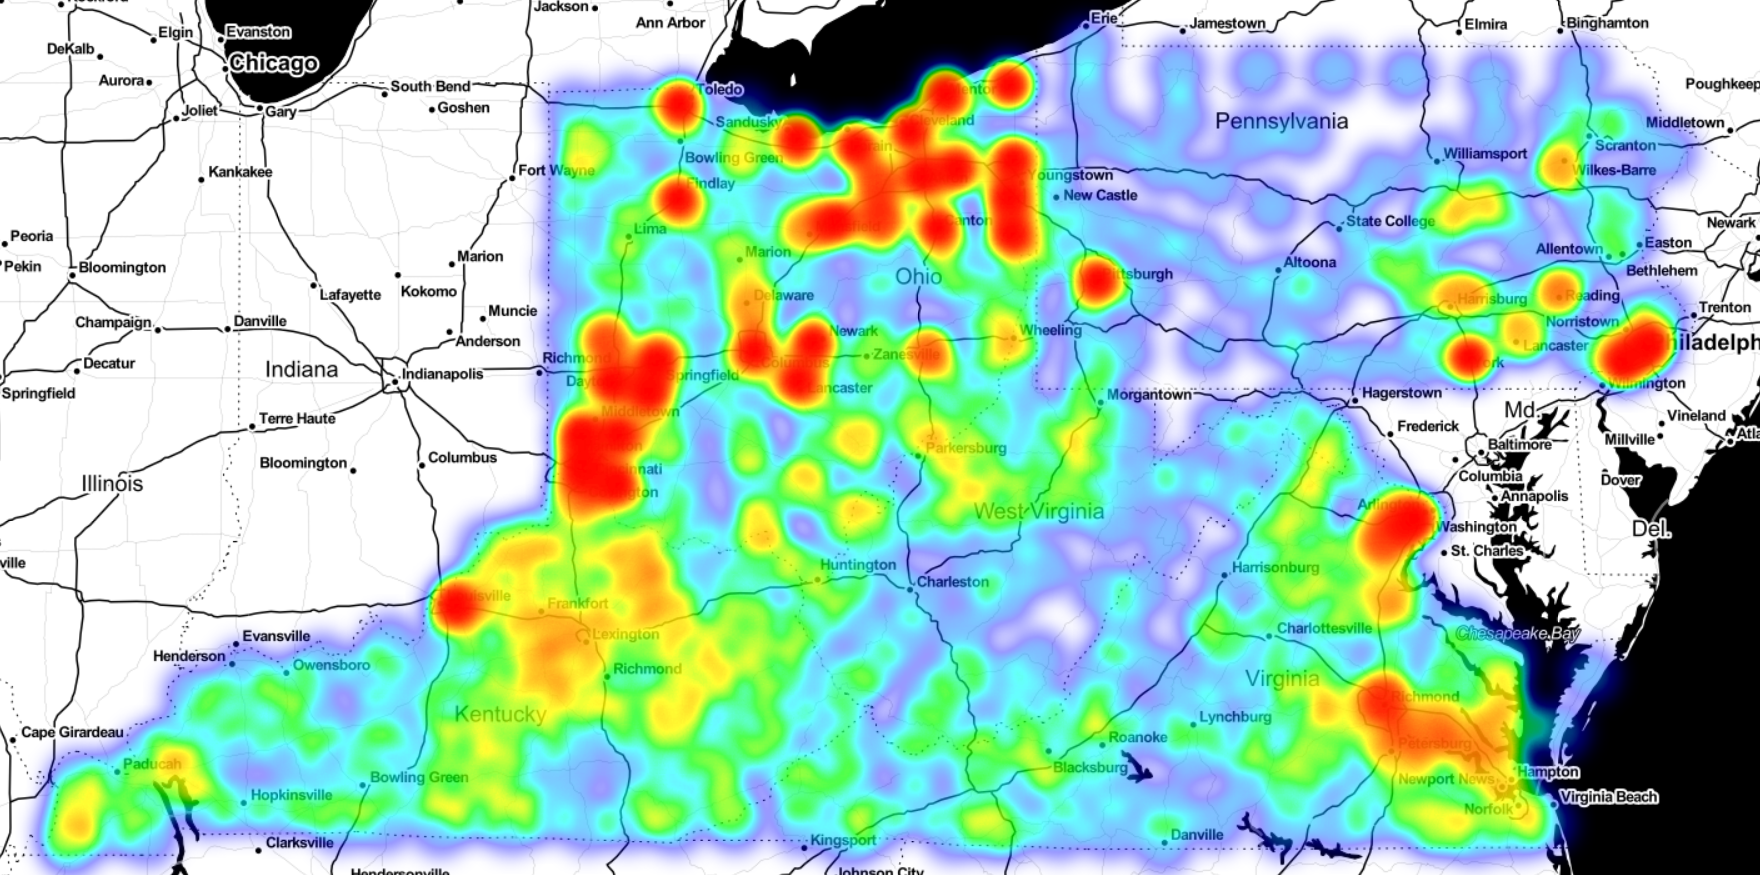
\includegraphics[scale=0.13]{plots/prediction2025.png}
}
\subfigure[{Prediction 2030}]{
  \label{mb-state}
  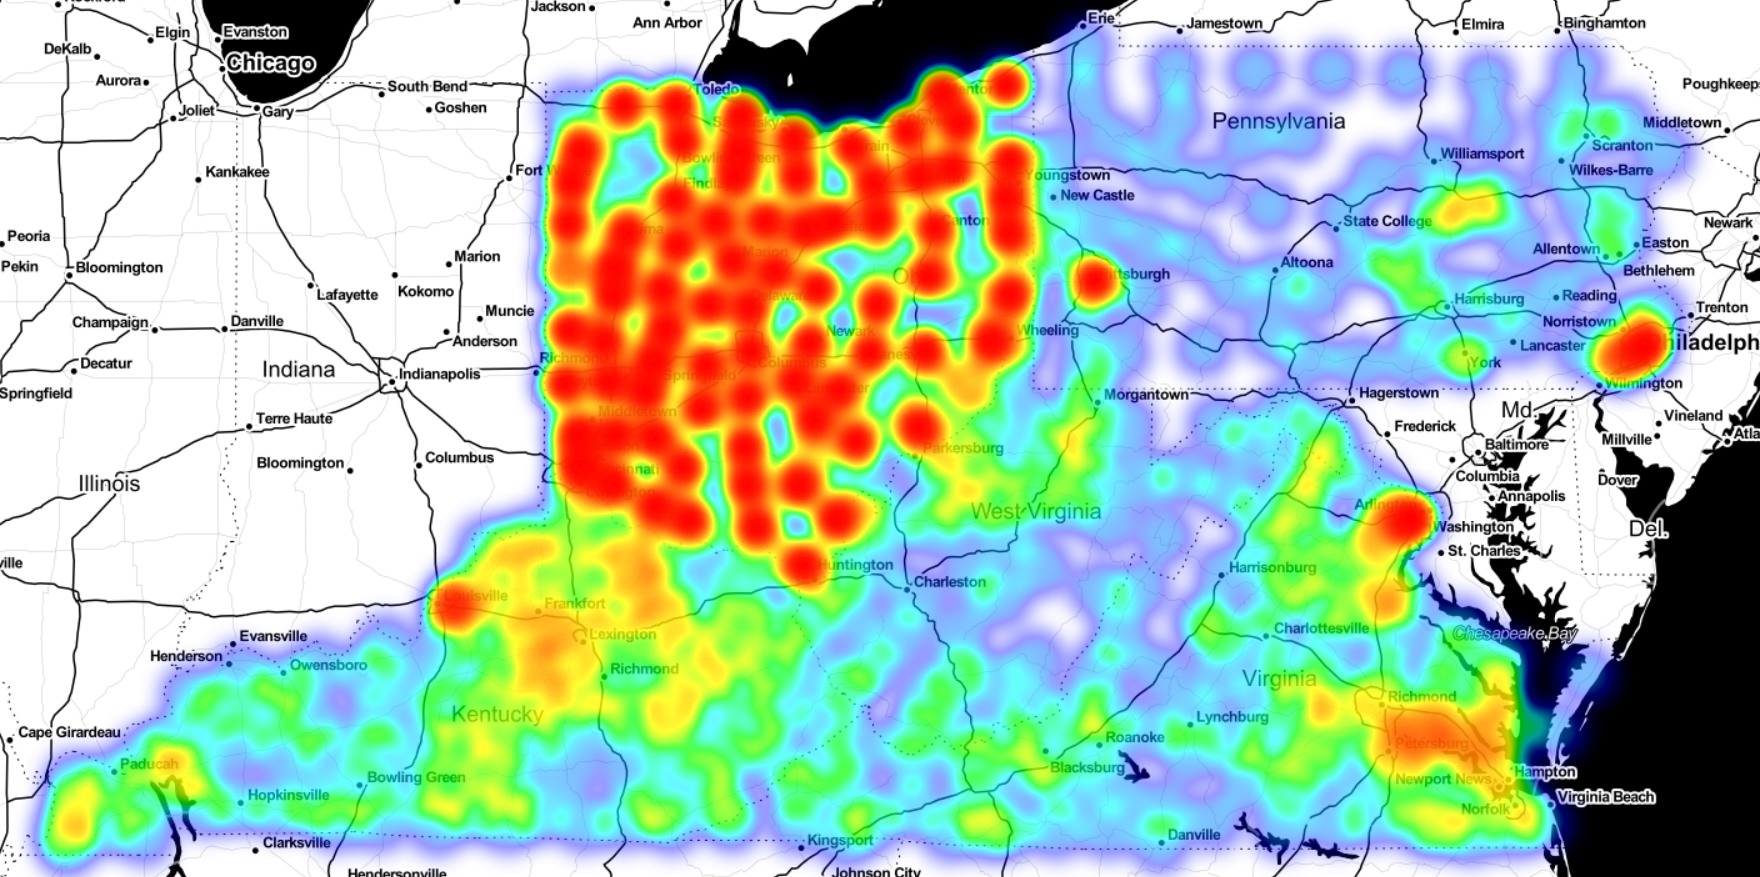
\includegraphics[scale=0.13]{plots/prediction2030.png}
}
\caption{Predictions}
\label{pre}
\end{figure}

As is shown in the heat map, we predict that the opioid cases will gradually gather in Ohio. In the other states, the count of opioid cases will be less relatively. 

\section{Correlation Analysis}
\subsection{Apriori Algorithm}
Apriori\cite{Apriori} is an algorithm for frequent item set mining and association rule learning, which can discover relations between variables, over transactional databases. It proceeds by identifying the frequent individual items in the database and extending them to larger and larger item sets as long as those item sets appear sufficiently often in the database. In our analysis, each set only consists an individual item. The frequent item sets determined by Apriori can be used to determine association rules which highlight general trends in the database. As a result, we can consider the relation between $P_d$ and each item, identify what kind of people are using opioids, and discover which variables are more likely to contribute to the growth in opioids use and addiction. 

We regard an item set A as frequent if it support $S_A$ is over 0.05. $S_A$ is defined as the proportion of records that contain the item set A in the dataset. Confidence $C_{A \to B}$ means the probability of B's occurrence under the condition of A's occurrence. We regard an item set B is associated strongly with another item set A if $C_{A \to B}$ is over 0.3. The value of $C$ is determined by the following three steps:
\begin{itemize}
\item Suppose AB is the item set which contains both A and B, $N$ is the number of A's occurrence, $n$ is the number of AB's occurrence, $S_B$ equals to 0.25. If B is independent of A, then $C_{A -> B}$, or $S_{B|A}$ as the same, also equals to 0.25. 
\item If we want to test the association between A and B, our test can be
\[H_0: C_{A \to B} = 0.25 \text{\quad against \quad} H_1: C_{A \to B} > 0.25 \text{.}\]
\item We can know that n follows a Binomial distribution $Bin(N, 0.25)$ under $H_0$, and $N$ is at least 23 since our dataset has 460 data and $S_A$ is over 0.05. If we can reject $H_0$ at the 20\% significant level, which means that B is associated strongly with A, the observed $n$ should at least be 7 and as a result $C_{A -> B}$ should be at least 0.304.
\end{itemize}

\subsection{Data Preprocessing}
We only consider the percentage of a variable and classify each variable according to its value into four categories("1","2","3","4"), in which "1", "2", "3" and "4" denotes the first, second, third and fourth quarter. Each category of certain variable is named as the variable's name combined with its rank. For example, $P_{os}$ of each county is classified into "drug\_1", "drug\_2", "drug\_3" and "drug\_4".

In our analysis, we are concerned about the item set B which contains the "1" or "4" category of $P_{os}$, and the item set A which contains the "1" or "4" category of other variables. Note that A and B both contain only one item.

We also compute each state's growth rate of $P_{os}$ by linear regression. The trend of $P_{os}$ for each state is like \textbf{Figure \ref{rate}} and the coefficients are like \textbf{Table \ref{coef}}. Since the uncertainty of VA is too large, we don't take it into consideration in the following analysis. All growth rates which appear in the following subsections are determined by the same method. 
 
\begin{figure}[h]
\centering
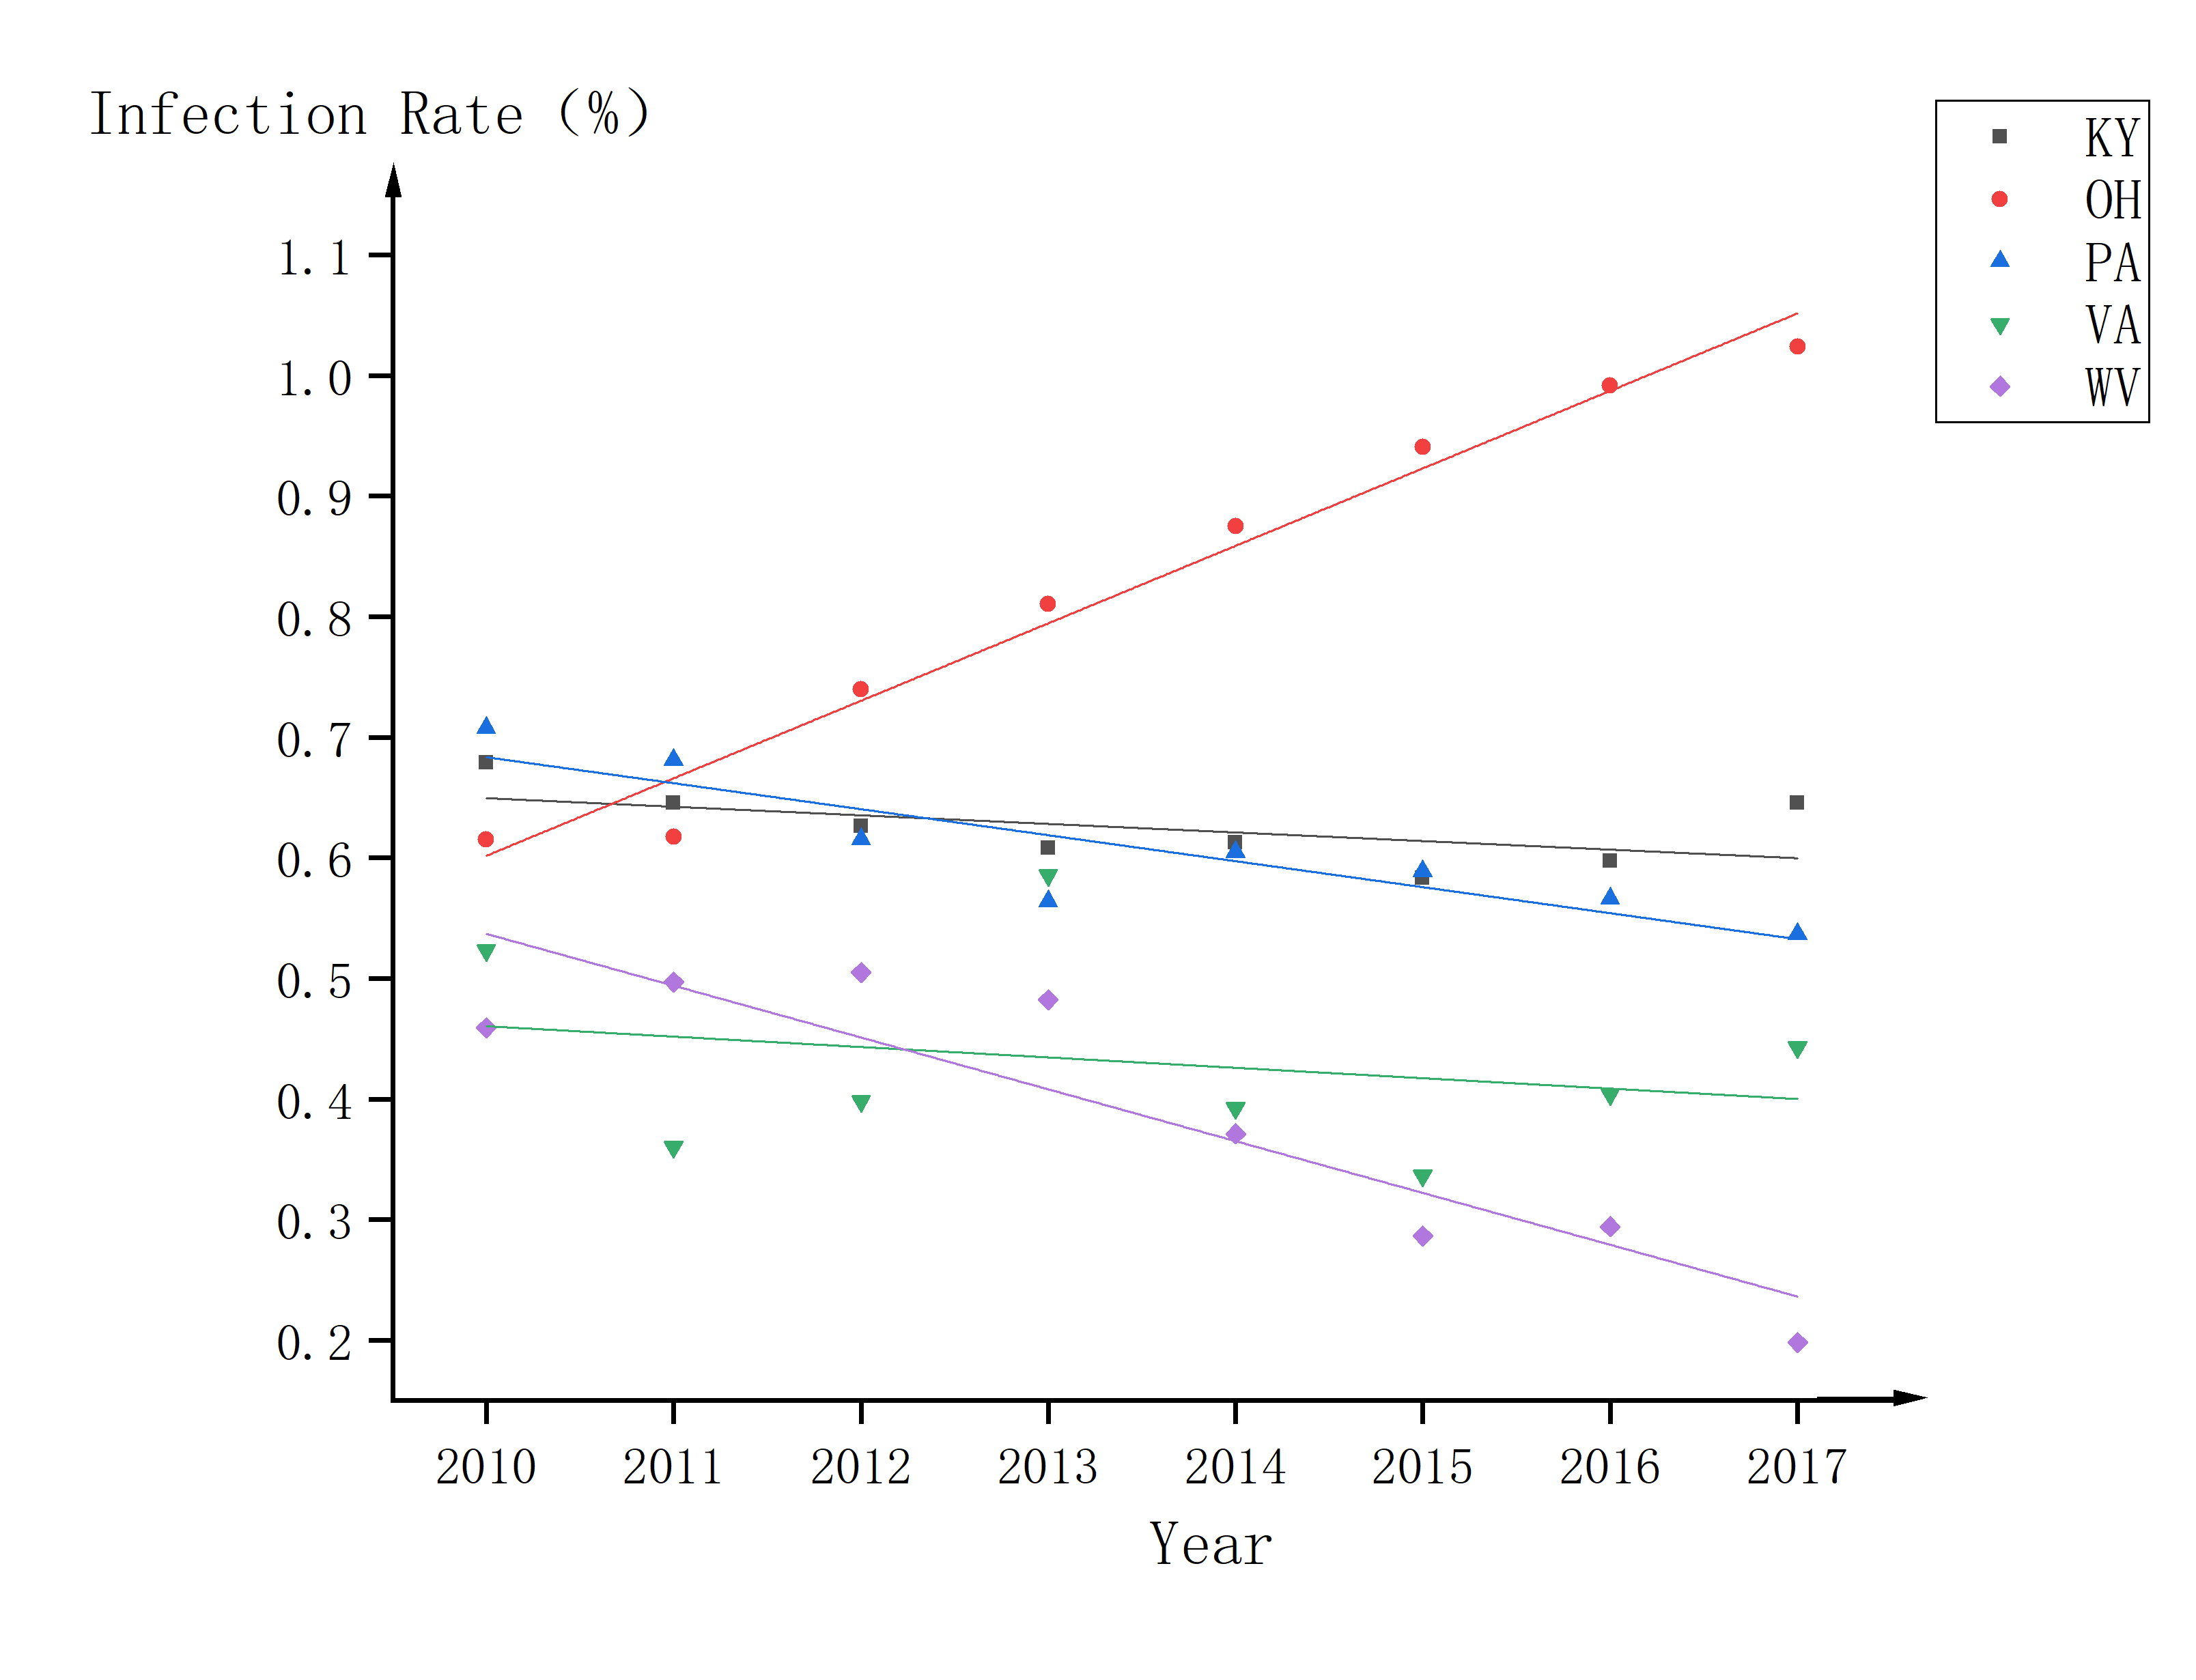
\includegraphics[width=10cm]{plots/rate.png}
\caption{$G_{p,os}$}
\label{rate}
\end{figure}

\begin{table}[h]
\centering
\begin{tabular}{cccccc}
  \toprule
   & \multicolumn{5}{c}{State} \\
  \cmidrule{2-6}
& KY & OH & PA & VA & WV  \\
  \midrule
  Intercept & 0.28 $\pm$ 0.05 & -1.37 $\pm$ 0.09 & 0.45 $\pm$ 0.12 & 0.30 $\pm$ 0.36 & 0.76 $\pm$ 0.21  \\
  Slope & (-13.6 $\pm$ 3)E-5 & (68 $\pm$ 5)E-5 & (-22 $\pm$ 6)E-5 & (-1.5 $\pm$ 1.8)E-4 & (-3.8 $\pm$ 1.0)E-4  \\
  R square & 0.84 & 0.98 & 0.74 & 0.12 & 0.72  \\
  \bottomrule
\end{tabular}
\caption{Coefficients}
\label{coef}
\end{table}

\subsection{Results and Analysis}
\subsubsection{Results of the Apriori}
The result of Apriori for the year of 2010, 2013 and 2016 is like \textbf{Table \ref{result}}, which lists every item set A associated strongly with the item set B and its corresponding $C_{A \to B}$ in parenthesis. 

\begin{table}[h]
\centering
\begin{tabular}{cccc}
  \toprule
   & \multicolumn{3}{c}{drug\_1} \\
  \cmidrule{2-4}
& 2010 & 2013 & 2016  \\
  \midrule
  & HC03\_VC07\_4(0.430) & HC03\_VC010\_1(0.310) & HC03\_VC08\_1(0.313)  \\
  & HC03\_VC11\_1(0.433) & HC03\_VC011\_1(0.315) & HC03\_VC11\_1(0.318)  \\
  A($C_{A \to B}$) & HC03\_VC93\_4(0.430) & HC03\_VC08\_1(0.340) & HC03\_VC41\_1(0.331)  \\
  & HC03\_VC85\_1(0.437) & HC03\_VC201\_4(0.326) & HC03\_VC122\_1(0.338)  \\
  & HC03\_VC206\_4(0.395) & HC03\_VC208\_4(0.324) & HC03\_VC186\_1(0.331)  \\
  \bottomrule
\end{tabular}
\begin{tabular}{cccc}
  \toprule
   & \multicolumn{3}{c}{drug\_4} \\
  \cmidrule{2-4}
& 2010 & 2013 & 2016  \\
  \midrule
  & HC03\_VC07\_1(0.336) & HC03\_VC010\_4(0.480) & HC03\_VC08\_4(0.393)  \\
  & HC03\_VC11\_4(0.439) & HC03\_VC011\_4(0.455) & HC03\_VC11\_4(0.365)  \\
  A($C_{A \to B}$) & HC03\_VC206\_1(0.305) & HC03\_VC08\_4(0.511) & HC03\_VC41\_4(0.424)  \\
  & HC03\_VC189\_1(0.376) & HC03\_VC201\_1(0.407) & HC03\_VC122\_4(0.347)  \\
  & HC03\_VC187\_1(0.384) & HC03\_VC208\_1(0.337) & HC03\_VC186\_4(0.394)  \\
  \bottomrule
\end{tabular}
\caption{Associated Item Sets}
\label{result}
\end{table}

We select the variable which affects both "drug\_1" and "drug\_4" in each year and thus find out our variable of interest(VOI): "HOUSEHOLDS BY TYPE - Family households (families) - Married-couple family", "HOUSEHOLDS BY TYPE - Family households (families) - Male householder, no wife present, family", "HOUSEHOLDS BY TYPE - Family households (families) - Female householder, no husband present, family" and "HOUSEHOLDS BY TYPE - Family households (families) - Female householder, no husband present, family - With own children under 18 years". We summarize them into two features: married-couple families and separated-couple families, and then analyze them one by one in the following subsections.

\subsubsection{Analysis of Married-couple Families}
The variable of "HOUSEHOLDS BY TYPE - Family households (families) - Married-couple family" appears to be strongly associated with $P_{os}$ in 2010. We suppose A1 to be "HC03\_VC07\_4", A2 to be "HC03\_VC07\_1", B1 to be "drug\_1" and B2 to be "drug\_4". It can be found that $C_{A1 \to B1}$ equals to 0.430 and $C_{A2 \to B2}$ equals to 0.336 in 2010, which means that $P_d$ is strongly associated by the percent of married-couple families and the correlation is negative. 

Our plot of each state's absolute growth rate of the percentage of married-couple families is like \textbf{Figure \ref{m-state}}, and the states are ascendingly ordered by their $G_{p,os}$. Since it is not good enough, we then discover by reading literature that there is an education gap in marriage, which means adults with a four-year college degree are more likely to get married than adults with some college education and with no education beyond high school, although the three percentages of marriage are all decreasing.\cite{marriage} We think that adults with a four-year college degree are less likely to be addicted to opioids than the other two kinds of people, since they earn more and their strains of life are less, so we subtract the growth rate of adults with a bachelor's degree or higher $G_{p,b}$ from the absolute growth rate of marriage $G_{p,m}$ and thus get the offset in 2010-2016 for each state. Our plot of each state's offset is like \textbf{Figure \ref{mb-state}}, and the states are ascendingly ordered by their $G_{p,os}$. 

\begin{figure}[h]
\centering
\subfigure[{$G_{p,m}$}]{
  \label{m-state}
  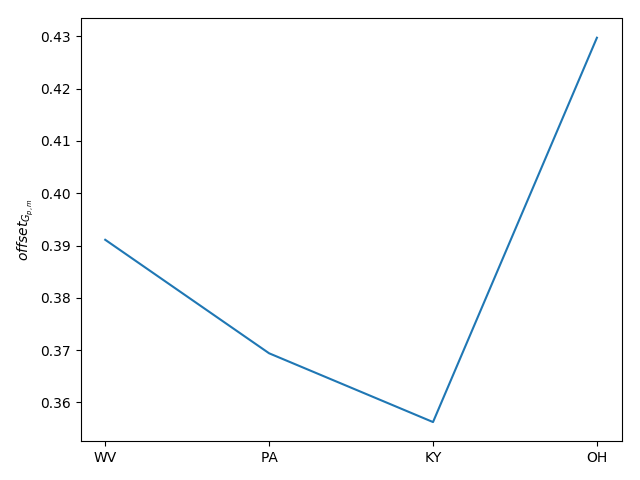
\includegraphics[scale=0.3]{plots/m-state.png}
}
\subfigure[{offset of $G_{p,m}$ and $G_{p,b}$}]{
  \label{mb-state}
  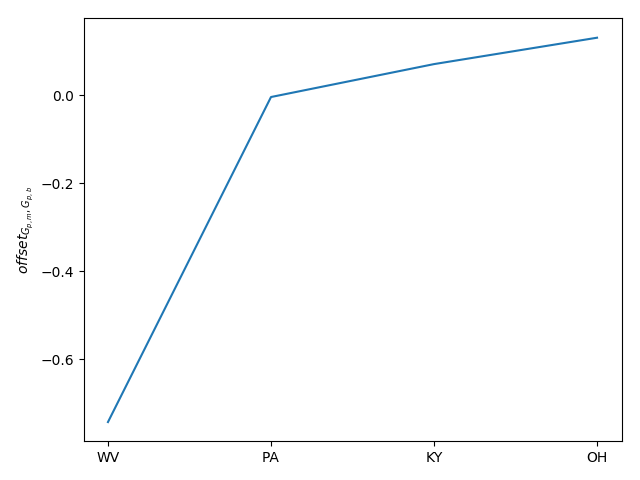
\includegraphics[scale=0.3]{plots/mb-state.png}
}
\caption{Married-couple Families}
\end{figure}

From the result, we can draw a conclusion that adults with some college education and with no education beyond high school who don't get married are likely to use/abuse opioids, and the growth of its percentage contributes to the  growth of the percentage of opioid use and addiction $G_{p,os}$.

\subsubsection{Analysis of Separated-couple Families}
The variable of "HOUSEHOLDS BY TYPE - Family households (families) - Male householder, no wife present, family" appears to be strongly associated with $P_d$ in 2013 and 2016. We suppose A1 to be "HC03\_VC08\_1", A2 to be "HC03\_VC08\_4", B1 to be "drug\_1" and B2 to be "drug\_4". It can be found that $C_{A1 \to B1}$ equals to 0.340 and $C_{A2 \to B2}$ equals to 0.511 in 2013, and that $C_{A1 \to B1}$ equals to 0.313 and $C_{A2 \to B2}$ equals to 0.393 in 2016, which means that $P_{os}$ is strongly associated by the percent of married-couple families and the correlation is positive. 

The variable of "HOUSEHOLDS BY TYPE - Family households (families) - Female householder, no husband present, family" appears to be strongly associated with $P_{os}$ in 2010, 2013 and 2016. We suppose A1 to be "HC03\_VC11\_1", A2 to be "HC03\_VC11\_4", B1 to be "drug\_1" and B2 to be "drug\_4". It can be found that $C_{A1 \to B1}$ equals to 0.433 and $C_{A2 \to B2}$ equals to 0.439 in 2013, $C_{A1 \to B1}$ equals to 0.315 and $C_{A2 \to B2}$ equals to 0.455 in 2013, and that $C_{A1 \to B1}$ equals to 0.318 and $C_{A2 \to B2}$ equals to 0.365 in 2016, which means that $P_{os}$ is strongly associated by the percent of married-couple families and the correlation is positive. 

The variable of "HOUSEHOLDS BY TYPE - Family households (families) - Female householder, no husband present, family - With own children under 18 years" appears to be strongly associated with $P_{os}$ in 2016. We suppose A1 to be "HC03\_VC10\_4", A2 to be "HC03\_VC10\_1", B1 to be "drug\_1" and B2 to be "drug\_4". It can be found that $C_{A1 \to B1}$ equals to 0.310 and $C_{A2 \to B2}$ equals to 0.480 in 2013, which means that $P_{os}$ is strongly associated by the percent of married-couple families and the correlation is negative. 

We substract the growth rate of the percentage of female householder, no husband present, families with own children under 18 years(which is positive) from the growth rate of the percentage of separated-couple families(which is positive), which contain both male householder, no wife present, families and female householder, no husband present, families and thus get the offset in 2010-2016 for each state. Our plot of each state's offset is like \textbf{Figure \ref{nw,nh,nhc-state}}, and the states are ascendingly ordered by their $G_{p,os}$.

\begin{figure}[h]
\centering
\subfigure[{offset of $G_{p,nw}$, $G_{p,nh}$ and $G_{p,nhc}$}]{
  \label{nw,nh,nhc-state}
  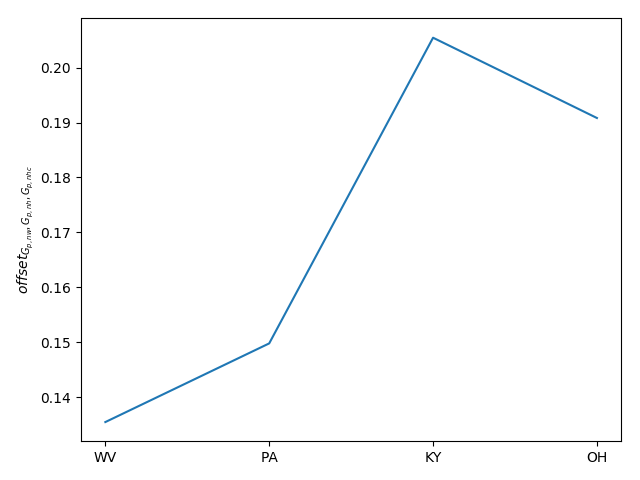
\includegraphics[width=8cm]{plots/nw,nh,nhc-state.png}
}
\caption{Separated-couple Families}
\end{figure}

From the result, we can draw a conclusion that men with no wife present and women with no husband and own children present are likely to use/abuse opioids, and the growth of its percentage contributes to the growth of the percentage of opioid use and addiction $G_{p,os}$.

\section{Model Modification Based on Mined Factors}


\section{Sensitivity Analysis}


\section{Strategies and Evaluation}


\section{Conclusion}
\subsection{Strengths and Weaknesses}
\subsubsection{Strengths}
\begin{itemize}
    \item First one...
    \item Second one ...
\end{itemize}
\subsubsection{Weaknesses}
\begin{itemize}
    \item Only one ...
\end{itemize}
 
\subsection{Future Work}

\bibliographystyle{unsrt}
\addcontentsline{toc}{section}{References}  %引用部分标题("Refenrence")的重命名
\bibliography{video_senti_v2}



% ==============以下为附录内容,如您的论文中不需要程序附录请自行删除====================
\clearpage
\begin{subappendices}						% 附录环境
\section*{Apendix: The source codes}		% 附录标题可以自行修改
\addcontentsline{toc}{section}{Appendix}  	% 将附录内容加入到目录中

This MATLAB program is used to calculate the value of variable $a$.
\begin{lstlisting}[language=Matlab, caption=\texttt{temp.m}]
a = 0;
for i = 1:5
	a = a + 1;
end
\end{lstlisting}

This LINGO program is used to search the optimize solution of 0-1 problem.
\begin{lstlisting}[language=Lingo, caption=\texttt{temp.lg4}]
model:
sets:
WP/1..12/: M, W, X;
endsets
data:
M = 2 5 18 3 2 5 10 4 11 7 14 6;
W = 5 10 13 4 3 11 13 10 8 16 7 4;
enddata
max = @sum(WP:W*X);
@sum(WP: M * X)<=46;
@for(WP: @bin(X));
end
\end{lstlisting}

\end{subappendices}
% =================================================================================



\end{document}